\subsubsection{Nation Drop-Down}
    In the nation drop-down button as shown in figure \ref{figure-nation-drop-down}, if user choose one of the lists as shown in figure \ref{figure-nation-lists}, it will be sent the value to the server which that the server will pass the nation filter to match that which type that user choose. Then it will get the the code of the country such as Thailand is 099, Myanma is 048, Laso is 056, and Cambodia is 057, in order to correctly count people in each nation depending on the nation filter.
    
% Thai = 099
%   val MYANMA: String = "048"
%   val LAOS: String = "056"
%   val CAMBODIA: String = "057"

    \FloatBarrier
        \begin{figure}[h!]
            \centering
                % can use width=\linewidth
        		
\includegraphics[width=\linewidth]{images/chapter-06/nation-1.png}
            	\caption{Nation Drop-Down}
        		\label{figure-nation-drop-down}
        \end{figure}
    \FloatBarrier
    
    \FloatBarrier
        \begin{figure}[h!]
            \centering
                % can use width=\linewidth
        		
\includegraphics[width=\linewidth]{images/chapter-06/nation-2.png}
            	\caption{Nation Lists}
        		\label{figure-nation-lists}
        \end{figure}
    \FloatBarrier
    
\subsubsection{Time Drop-Down}  

    
    In time drop-down button as shown in figure \ref{figure-time-drop-down}, there are three different type of it that user can choose as shown in figure \ref{figure-time-lists}. First, if user chooses all, it means that the server will choose time at the beginning of the data until the end of the data. The beginning here mean the first date of the data and the 23:59 of the end of the data. Second, if user chooses time-interval as shown in figure \ref{figure-time-interval-drop-down}, it means the server will choose the first date of the starting month, and follow by the month and the year that user choose to be the starting date time. Then it will end up at the end date of that month, the month and year that user choose as shown in figure \ref{figure-time-interval-drop-down}Third, if user chooses cut-off time as shown in figure  \ref{figure-time-end-date-drop-down}, it means that the server will choose the starting date at the beginning of the data and it will end up at the end date of the month that user choose, month, and year that user choose as shown in figure \ref{figure-time-end-date-drop-down}. In addition, the beginning date means that will pick the start of the date. for example if user choose first month and 2017, it means that the server will choose 1/1/2017. Unlike the beginning date, the end date will choose the last first of the date that pick, for instance, if user choose end date as second month and 2017, the server will choose 31/1/2017 at time 23:59.9.
    

    \FloatBarrier
        \begin{figure}[h!]
            \centering
                % can use width=\linewidth
        		
\includegraphics[width=9cm]{images/chapter-06/time-all.png}
            	\caption{Time Drop-Down}
        		\label{figure-time-drop-down}
        \end{figure}
    \FloatBarrier
    
    \FloatBarrier
        \begin{figure}[h!]
            \centering
                % can use width=\linewidth
        		
\includegraphics[width=9cm]{images/chapter-06/time-lists.png}
            	\caption{Time Lists}
        		\label{figure-time-lists}
        \end{figure}
    \FloatBarrier
    
    \FloatBarrier
        \begin{figure}[h!]
            \centering
                % can use width=\linewidth
        		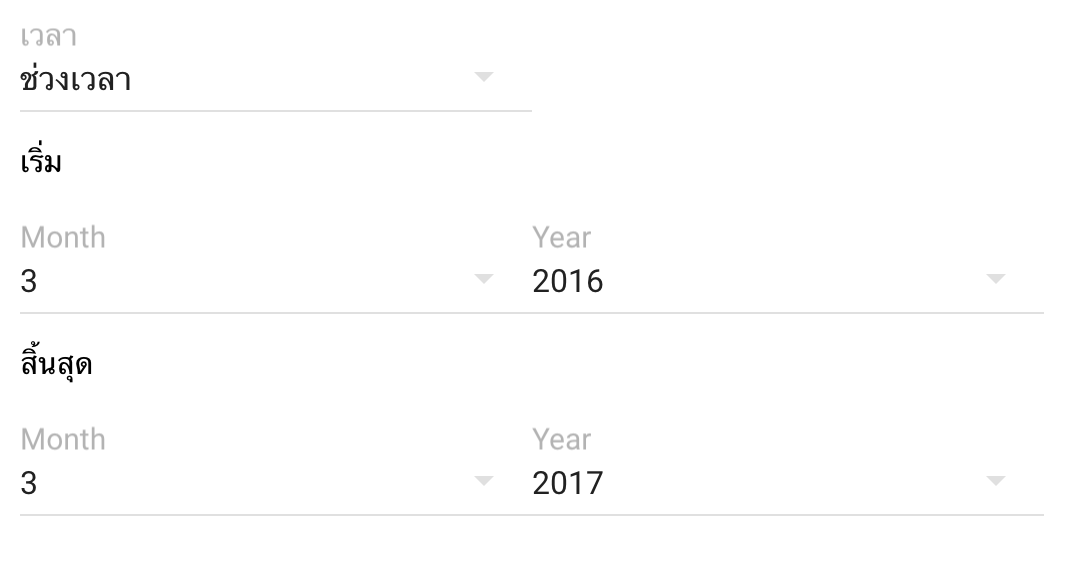
\includegraphics[width=\linewidth]{images/chapter-06/time-interval.png}
            	\caption{Time Interval Drop-Down}
        		\label{figure-time-interval-drop-down}
        \end{figure}
    \FloatBarrier
    
    \FloatBarrier
        \begin{figure}[h!]
            \centering
                % can use width=\linewidth
        		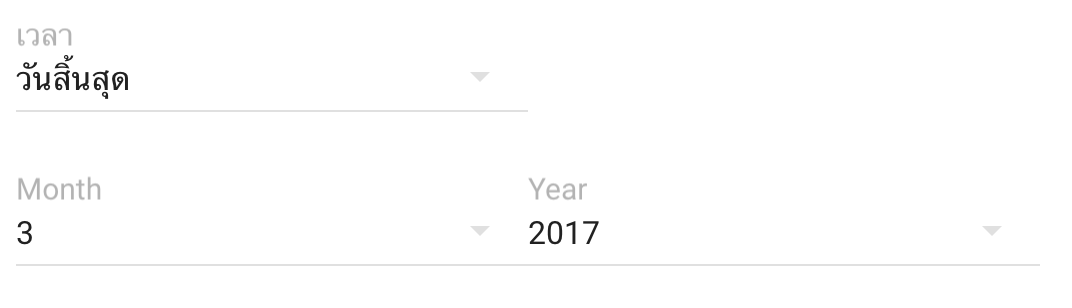
\includegraphics[width=\linewidth]{images/chapter-06/time-end-date.png}
            	\caption{Time End Date Drop-Down}
        		\label{figure-time-end-date-drop-down}
        \end{figure}
    \FloatBarrier
    
\subsubsection{Disease and Criteria Drop-Down}
    In disease and criteria drop-down button as shown in figure \ref{figure-disease-drop-down} and \ref{figure-disease-lists}, there are for different type of diseases that user can choose. Also in each disease there are many criteria that user can choose. It means that criteria will change according to the disease as shown in figure \ref{figure-disease-lists}. First, if user choose HIV, the criteria will show as in figure \ref{figure-disease-hiv-lists}, "All" means that choosing both HIV confirmed and HIV presumed. HIV confirmed means that patient who have diagnosis result (Z21, B20X, B21X) by the doctor and HIV presumed means that patient who receiving antiviral drug more than two types. "Confirmed" means choosing only HIV confirmed, and "HIV TB Comorbidity" means the server will choose patient that have HIV all and also the patient should have TB.
    % ?? "HIV TB" ==> which type of hiv(confirm or all)
    
    Second, if user choose Hepatitis C, the criteria will show as in figure \ref{figure-disease-hepatitis-c-lists}, "All" means choosing all patient that have diagnosis test in the criteria of hepatitis C. "Acute" means patient that has the diagnosis result of (B171, B1710, B1711) by the doctor and can be cured by the drug. "Chronic" means choosing the patient from the diagnosis result of (z2252,B182,B192,B1920,B1921) and this is the stage 2 that develop from acute if there is no drug action taken. It is when virus damages the liver enough to cause the signs and symptoms of liver disease. "Cirrhosis" means choosing the patient from the diagnosis result of (K743,K744,K745,K746) and have the previous diagnosis result in range of hepatitis C. Cirrhosis happen when the patient have permanent scar tissue replaces healthy liver cells from the virus of hepatitis C. "Hepatocellular Carcinoma" means the diagnosis result of the patient is C220 and have the previous diagnosis result in range of hepatitis C. It is a dead stage where patient need surgery as the hepatitis C virus developed to become the cancer.
    
    Third, if user choose Hepatitis B, the criteria will show as in figure \ref{figure-disease-hepatitis-d-lists}, All" means choosing all patient that have diagnosis test in the criteria of hepatitis B. "Acute" means choosing the patient that get the diagnosis result of (B160,B161,B162,B169) and can be cured by drug. "Chronic" means choosing the patient that has the diagnosis result of (Z2251,B180,B181,B191,B1910,B1911). Chronic hepatitis B is a development from acute stage of hepatitis B where there is no treatment taken place. "Acute With HDV" means the patient has the diagnosis of B160 or B161. It only happen to the patient who carry hepatitis B to be infect by HDV or Delta agent (Hepatitis D) and make the symptom of the patient get worse. "Chronic With HDV" means choosing the patient from the diagnosis result of B180 and the patient are infect to hepatitis D after carry the hepatitis B virus. "Cirrhosis" has the same diagnosis result as same as cirrhosis in hepatitis C but cause from the hepatitis B instead. "Hepatocellular Carcinoma" means choosing the patient diagnosis result of C220 and have the previous diagnosis result in the type of hepatitis B. It is the stage where the virus become cancer and patient need to surgery.
    
    Lastly, if user choose TB, There is only one criteria in this field which is "All". It means patient who have TB.
    
    
    \FloatBarrier
        \begin{figure}[h!]
            \centering
                % can use width=\linewidth
        		
\includegraphics[width=9cm]{images/chapter-06/disease.png}
            	\caption{Disease Drop-Down}
        		\label{figure-disease-drop-down}
        \end{figure}
    \FloatBarrier
    
    \FloatBarrier
        \begin{figure}[h!]
            \centering
                % can use width=\linewidth
        		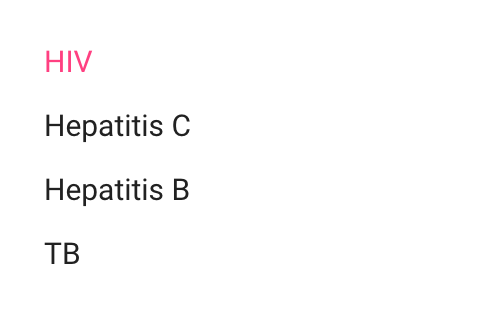
\includegraphics[width=9cm]{images/chapter-06/disease-lists.png}
            	\caption{Disease Lists}
        		\label{figure-disease-lists}
        \end{figure}
    \FloatBarrier
    
    \FloatBarrier
        \begin{figure}[h!]
            \centering
                % can use width=\linewidth
        		
\includegraphics[width=9cm]{images/chapter-06/disease-hiv-lists.png}
            	\caption{HIV Lists}
        		\label{figure-disease-hiv-lists}
        \end{figure}
    \FloatBarrier
    
    \FloatBarrier
        \begin{figure}[h!]
            \centering
                % can use width=\linewidth
        		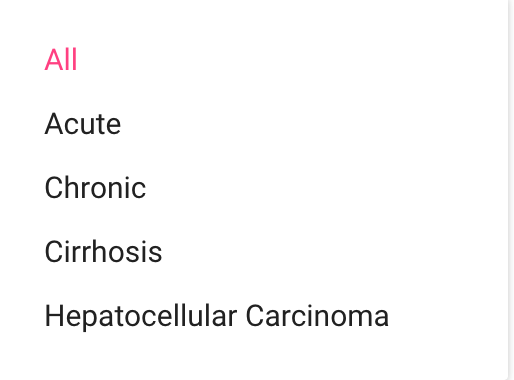
\includegraphics[width=9cm]{images/chapter-06/disease-hepatitis-c-lists.png}
            	\caption{Hepatitis C Lists}
        		\label{figure-disease-hepatitis-c-lists}
        \end{figure}
    \FloatBarrier
    
    \FloatBarrier
        \begin{figure}[h!]
            \centering
                % can use width=\linewidth
        		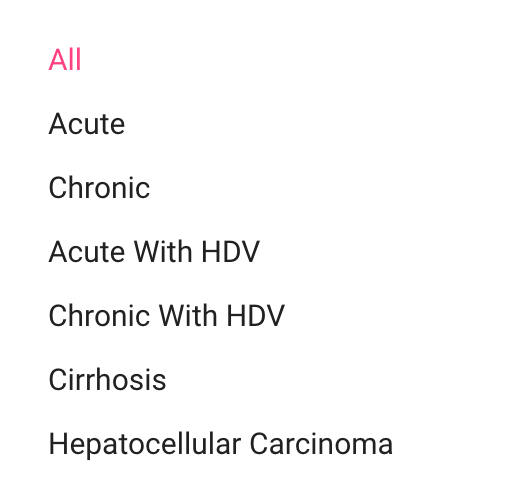
\includegraphics[width=8cm]{images/chapter-06/disease-hepatitis-d-lists.png}
            	\caption{Hepatitis B Lists}
        		\label{figure-disease-hepatitis-d-lists}
        \end{figure}
    \FloatBarrier


\subsubsection{Type of Report Dropdown}


    
    
    In type of report drop-down button as shown in figure \ref{figure-type-of-report-drop-down}, there are four different type of it that user can choose as shown in figure \ref{figure-type-of-report-lists}. First, if user chooses "Country", it means that the server will select all hospitals. Second, if user chooses "Area", it will pop-up area drop-down as shown in figure \ref{figure-type-of-report-area}, it means that the server will select the data according to the area that user choose. Third, if user chooses "Province" it will pop-up area drop-down and province drop-down  as shown in figure \ref{figure-type-of-report-province}, it means that the server will choose the data according to the province that user choose. Before user choose the province, the list of the province will be picked from the area that user choose. Lastly, if user chooses "Hospital" it will pop-up area drop-down, province drop-down, and hospital drop-down  as shown in figure \ref{figure-type-of-report-hospital}, it means that the server will choose the data according to the hospital that user choose. Like choosing "Province", the list of hospital will be picked from the province that user choose and the list of province will be picked according to the area that user choose.

    

    \FloatBarrier
        \begin{figure}[h!]
            \centering
                % can use width=\linewidth
        		
\includegraphics[width=9cm]{images/chapter-06/type-of-report-all.png}
            	\caption{Type of Report Drop-Down}
        		\label{figure-type-of-report-drop-down}
        \end{figure}
    \FloatBarrier
    
    \FloatBarrier
        \begin{figure}[h!]
            \centering
                % can use width=\linewidth
        		
\includegraphics[width=9cm]{images/chapter-06/type-of-report-lists.png}
            	\caption{Type of Report Lists}
        		\label{figure-type-of-report-lists}
        \end{figure}
    \FloatBarrier
    
    \FloatBarrier
        \begin{figure}[h!]
            \centering
                % can use width=\linewidth
        		
\includegraphics[width=\linewidth]{images/chapter-06/type-of-report-area.png}
            	\caption{Type of Report (Area Drop-Down)}
        		\label{figure-type-of-report-area}
        \end{figure}
    \FloatBarrier
    
    \FloatBarrier
        \begin{figure}[h!]
            \centering
                % can use width=\linewidth
        		
\includegraphics[width=\linewidth]{images/chapter-06/type-of-report-province.png}
            	\caption{Type of Report (Province Drop-Down)}
        		\label{figure-type-of-report-province}
        \end{figure}
    \FloatBarrier
    
    \FloatBarrier
        \begin{figure}[h!]
            \centering
                % can use width=\linewidth
        		
\includegraphics[width=\linewidth]{images/chapter-06/type-of-report-hospital.png}
            	\caption{Type of Report (Hospital Drop-Down)}
        		\label{figure-type-of-report-hospital}
        \end{figure}
    \FloatBarrier



